\chapterimage{/8/head.jpg} % Chapter heading image
\chapter{Statistica con un oggetto}\label{8:ch}

\section{Proprietà Stocastiche delle Perturbazioni}
L'approccio statistico all'analisi delle perturbazioni si basa sulla quantità: $\delta (\vec{x}) = \left (\rho(\vec{x})-\overline{\rho} \right)/\overline{\rho}$ definibile per ogni punto dell'universo, ma della quale interessano principalmente le propietà medie. Il campo $\delta (\vec{x})$ deve essere invariante per traslazioni e rotazioni in base ai principi di omogeneità e isotropia. Da un punto di vista fisico, il campo è generato alla fine della fase inflazionaria (spiraleggiamento nel piano $\phi,\dot{\phi}$) da fluttuazioni statistiche della metrica (verrà assunto rumore bianco). Pertanto il valore $\delta (\vec{x_1})$ non è correlato in fase con $\delta (\vec{x_2})$ e la distribuzione dei valori di $\delta$ può essere assunta \textit{pressoché} gaussiana. Le rappresentazioni nello spazio di Fourier di questi campi, determinano una quantità fondamentale: $\langle \delta k^2 \rangle $.

Ipotesi ergodica: non potendo fare le medie su tante realizzazioni dell'universo (ne esiste una sola), le si fanno su sottospazi sufficientemente grandi e separati (tali da essere indipendenti, \textit{fair sample}) dell'unica realizzazione. Si può dimostrare che per una distribuzione gaussiana, l'ipotesi ergodica è un teorema. Oggi un \textit{fair sample} per avere omogeneità e isotropia si raggiunge a raggi $\gtrsim 100$ Mpc, questa scala diminuisce col tempo essendo l'universo meno strutturato. 

Una gaussiana $P(\delta)$ è definita univocamente da media e varianza, tutti i momenti dispari sono nulli e tutti i momenti pari sono potenze della varianza. Per definizione $\langle \delta \rangle =0 $. Il valore $\delta$ viene espresso nello spazio di Fourier:
\begin{equation}
    \delta{(\vec{x})}=\frac{1}{(2\pi)^3}\int \delta{(\vec{k})}\; e^{i\vec{k}\cdot\vec{x}}\; \d{^3 \vec{k}} \qquad \longleftrightarrow \qquad \delta{(\vec{k})}=\int \delta{(\vec{x})}\; e^{-i\vec{k}\cdot\vec{x}}\; \d{^3 \vec{x}}
\end{equation}
dove $k=2\pi/\lambda$, $\delta{(\vec{x})}$ è adimensionale, $k=[L^{-1}]$ e $\delta{(\vec{k})}=[L^3]$. Essendo un contrasto di densità, è necessario che $\delta{(\vec{x})}\in \mathbb{R} $, per cui per $\delta{(\vec{k})}\in\mathbb{C} $ deve valere: $\delta^*(\vec{k})=\delta{(-\vec{k})}$. Verranno ora introdotte alcune definizioni strategiche.

\vspace{2em}
\begin{example}[Delta di Dirac tridimensionale]
    (\textit{eh iniziamo ad avere troppi delta, ma dopotutto come potremmo chiamarla diversamente?})
    \begin{equation}
        \delta_D^{(3)}(k)= \frac{1}{(2\pi)^3} \int e^{-i\vec{k}\cdot\vec{x}}\; \d{^3 \vec{x}}\qquad \rightarrow\qquad \int f(\vec{k}) \delta_D^{(3)}( \vec{z}-\vec{k} )\d{^3 \vec{k}}= f(\vec{z})
    \end{equation}
\end{example}

\begin{example}[Funzione di correlazione a due punti]
    Indica come il campo correla con sé stesso (\textit{autocorrelazione}) in punti che distano $\vec{r}$ tra loro. È una media su tutti i punti dell'universo e su tutte le direzioni, infatti si sottintende che $\vec{r}=r\hat{n}$ (principio di isotropia). Questo sarà l'osservabile statistico principale per studiare il clustering.
    \begin{equation}
        \xi (r) := \langle\delta (\vec{x}) \delta(\vec{x}+\vec{r}) \rangle 
    \end{equation}
    \begin{equation}
        \xi (r)= \frac{1}{(2\pi)^6}\int \d{^3\vec{k}}\int \d{^3\vec{k'}}\; \langle \delta (\vec{k}) \delta(\vec{k'})\rangle \; e^{ik(\vec{x}+\vec{r})}\; e^{i\vec{k'}\cdot \vec{x}}\label{eq:8xi}
    \end{equation}
\end{example}
Da cui si deriva la teza definizione fondamentale.

\begin{example}[Spettro di potenza]

    \begin{equation}
        \mathcal{P}(k): \quad \langle \delta (\vec{k}) \delta(\vec{k'})\rangle = (2\pi)^3 \mathcal{P}(k)\; \delta_D^{(3)}(\vec{k}+\vec{k'})\label{eq:8pi}
    \end{equation}
    Anche riscrivibile utilizzando la richiesta: $\delta^*(\vec{k})=\delta{(-\vec{k})}$. A differenza della $\xi(r)$, questa quantità è definita nello spazio di Fourier. Inserendola nell'Equazione (\ref{eq:8xi}) si ottiene:
    \begin{equation}
        \xi (r) = \frac{1}{(2\pi)^3} \int \d{^3\vec{k}}\; \mathcal{P}(k)\; e^{i\vec{k'}\cdot \vec{r}}
    \end{equation}
    Questa relazione rappresenta il \textbf{teorema di Wiener–Khintchine}: la funzione di correlazione a due punti $\xi (r)$  e lo spettro di potenza $\mathcal{P}(k)$ sono una coppia di Fourier. Pur essendo $\xi (r)$ più facile da maneggiare in quanto appartenente allo spazio reale, $\mathcal{P}(k)$ è legato al $\delta (k)$ studiato nella teoria lineare e pertanto non se ne scampa. Infatti si può osservare che: $\mathcal{P}(k)\propto \langle\delta^2 (\vec{k})  \rangle $, ossia all'ampiezza quadratica media dell'onda con vettore d'onda $\vec{k}$. Volendo essere rigorosi, è una densità di potenza, la \textbf{potenza delle fluttuazioni} è adimensionale e vale: $\mathcal{P}(k)\d{^3 \vec{k}}$.
\end{example}

Come accennato in precedenza, per principio di isotropia, è conveniente passare alle coordiate sferiche, ricordandosi che $\int \d{^3 \vec{k}}=\int_0^{2\pi}\d{\varphi}\int_0^\pi\d{\theta}\sin\theta\int_0^\infty k^2\d{k}$. La relazione \ref{eq:8pi} modificata per $k=k'$ diventa:
\begin{equation*}
    \langle | \delta_k |^2 \rangle = (2\pi)^3 \; \mathcal{P}(k) \; \delta_D^{(3)}(0) = \mathcal{P}(k) \; V_\infty 
\end{equation*}
dove $V_\infty$ è il \textit{volume infinito}, un infinito formale che rappresenta l'intero volume di integrazione, il volume su tutto lo spazio. Pertanto si ha:
$$
\mathcal{P}(k)  \propto \langle | \delta_k|^2 \rangle
$$
Questo mostra, come precedentemente accennato, che lo spettro di potenza è legato al valore quadratico medio delle ampiezze delle perturbazioni sulla scala $k$. Nel caso di perturbazioni gaussiane, entra in gioco la varianza. 

\subsubsection*{Teorema di Parseval}
Siano $f$ e $g$ due funzioni a valori complessi in una dimensione, si ha che (dimostrabile dalle definizioni precedenti):
\begin{equation*}
    \int^{+\infty}_{-\infty} f(x)g^*(x)\d{x} = \frac{1}{2\pi} \int^{+\infty}_{-\infty} \widetilde{ f}(k)\widetilde{g}^*(k)\d{k}
\end{equation*}
Ossia l'integrale su tutto lo spazio reale del prodotto $f(x)g^*(x)$ è proporzionale all'integrale del prodotto delle due trasformate di Fourier. Per passare in tre dimensioni è sufficiente sostituire $2\pi\rightarrow (2\pi)^3$. 

\subsubsection*{Varianza del campo}
La varianza del campo di densità assunto gaussiano è: $\sigma^2 = \langle  \delta^2 (\vec{x}) \rangle$. Se si divide l'universo in regioni indipendenti e sufficientemente grandi da essere rappresentative, si può calcolare la varianza tramite una doppia media: la media su tutti i volumi della media spaziale quadratica di $\delta$:
\begin{equation*}
    \sigma^2 = \frac{1}{V_\infty} \int \langle  \delta^2 (\vec{x}) \rangle\; \d{^3\vec{x}} \qquad \rightarrow \qquad \sigma^2 = \frac{1}{(2\pi)^3} \int \mathcal{P}(\vec{k}) \; \d{^3\vec{k}}
\end{equation*}
Dove la seconda relazione è ottenuta con il Teorema di Parseval e rappresenta la \textbf{varianza puntuale}, ossia la somma dei contributi della potenza per ogni scala $k$ (è un'informazione globale/integrata). Da un punto di vista fisico è la potenza ricevuta complessivamente dal campo di densità. In coordinate sferiche diventa: $\sigma^2 =(2\pi)^{-1} \int  k^2\;\mathcal{P}(k)\; \d{k} $. 

Differentemente, $\delta (x)$ vorrebbe essere un'infomazione puntuale, ma provateci voi a calcolare la densità in un punto... non ha senso! Pertanto lo si fa mediandola entro un dato volume. La quantità è \textit{centrata} e non \textit{puntuale} e il campo si dice \textit{filtrato}.

\subsubsection*{Convoluzione}
Il ``filtraggio'' è svolto mediante l'operazione di convoluzione che è così definita:
\begin{equation*}
    [f*g](x) = \int_{-\infty}^{+\infty}f(x-y)g(y)\d{y}
\end{equation*}
Inoltre valgono le proprietà: $f*g=g*f$ e $h(x)=f*g\rightarrow h(k)=f\cdot g$, ossia l'operazione di convoluzione nello spazio di Fourier diventa un semplice prodotto. 

\subsection{Varianza di massa}
Nella pratica, per calcolare la densità, vanno definiti un punto e un raggio entro cui svolgere il conto. Inizialmente, si definisce il contrasto di massa dato una funzione filtro $W((\vec{x}),R)$ come:
$$
\frac{\delta M}{\overline{M}}(\vec{x}) = \delta_M(\vec{x}) = \delta (\vec{x}) * W(\vec{x}, R)
$$
$W$ (da \textit{window}) può essere top-hat $\sqcap $, gaussiano e così via. Questa quantità può essere ricondotta a conteggi di oggetti cosmici (o \textit{tracers}) entro un dato volume $V$:
$$
\frac{\delta N_t}{\overline{N_t}}(V) = \frac{N_t-\overline{N_t}(V)}{\overline{N_t}(V)}
$$
In genere si assume che la distribuzione dei traccianti sia una buona rappresentazione della distribuzione della materia oscura ivi presente. Per escludere effetti di feedback si usano prevalentemente gli ammassi di galassie. Nel caso delle galassie si introduce un fattore $b$ (\textbf{fattore di bias}) e si assume una relazione lineare tra le due quantità: $\delta_{N_g} = b \delta_M$.

Assumendo $\delta (\vec{x})$ gaussiano ($\Rightarrow \delta_M$ gaussiano) si può definire la \textbf{varianza di massa}:
\begin{equation}
    \sigma_M^2 :=  \langle  \delta_M ^2 \rangle = ... = \frac{1}{(2\pi)^3}\int \d{^3\vec{k}}\; \mathcal{P}(\vec{k}) \; W^2(\vec{k}, R)
\end{equation}
Un filtro di questo tipo è un passa-basso (cerca di livellare le disomogeneità tagliando le frequenze più alte). Aumentando la scala su cui si filtra ($R$), le disomogeneità locali (sulle frequenze più alte) vengono tagliate. Ossia, all'aumentare di $R$ passa meno segnale. In particolare si ha:
\begin{equation}
    \sigma_M^2 \xrightarrow[R\to 0]{} \sigma^2 \; (puntuale); \qquad \sigma_M^2 \xrightarrow[R\to \infty]{} 0 \label{eq8:sigmamvsr}
\end{equation}

È abbastanza chiaro che $R\propto k^{-1}\propto M^{1/3}$, quindi si può anche dire di filtrare una data massa.

\section{Spettro di potenza e relazioni di scala}
Si assume uno spettro di potenza del tipo $\mathcal{P}(k) = A k^{n}$, dove $n$ in questo caso è un indice spettrale di tipo scalare (le onde gravitazionali sono rappresentabili con un indice tensoriale). Per $n=0$ tutte le scale in $k$ hanno lo stesso valore di $\mathcal{P}(k)$, per $n>0$ i $k$ grandi (perturbazioni su scale piccole) hanno più potenza (ovvero, ci sono più disomogeneità sulle scale piccole). Questa forma degli spettri di potenza è detta \textit{scale-free}, non prevede scale privilegiate. Per questo motivo l'assunzione sarà valida solo per le condizioni iniziali, ossia in seguito all'inflazione.

La varianza puntuale per questo spettro può avere problemi di convergenza:
\begin{equation} \sigma^2 = \frac{A}{(2\pi)^2}\int_0^\infty  k^{2+n} \d{k} \quad converge \quad \leftrightarrow \quad n\; \left\{
    \begin{array}{ll}
    \leq -3 & k\rightarrow 0 \\
    \geq3 & k\rightarrow \infty
\end{array}\right.
\end{equation}

La varianza di massa diventa:
\begin{equation}
    \sigma_M^2 \propto \int \d{^3 \vec{k}}\; k^n\; W^2(k,R)
\end{equation}

Eventuali deviazioni dall'andamento di $\mathcal{P}(k)$ rispetto a quanto assunto, vengono visualizzate meglio con l'indice spettrale effettivo:
\begin{equation}
    n_{eff}=\frac{\d{\ln \mathcal{P}(k)}}{\d{\ln k}}
\end{equation}
che rappresenta in corrispondenza della scala $k$ la pendenza locale dello spettro.

\subsection{Relazioni di scala non lineari}\label{8:sec:relnlin}
Si può utilizzare la teoria lineare per predire i comportamenti delle relazioni di scala degli oggetti formati, che sono chiaramente in regime non lineare. In questo regime le perturbazioni evolvono con un fattore di crescita $\delta_+ (t)$ indipendente dalla scala, conseguentemente lo spettro iniziale verrà moltiplicato per un fattore $\delta_+^2 (t)$. Trascurando il filtro:
$$
\sigma_M^2 \quad\propto\quad \delta_+^2\; k^{n+3} \quad\propto\quad \delta_+^2\;  R^{-(n+3)} \quad\propto\quad \delta_+^2\;  M^{-(n+3)/3}
$$
La teoria lineare è valida finché $\sigma_M^2 \propto \delta^2 = 1$, per cui ponendo $\sigma_M^2 =1$ si definiscono le scale $k$ che diventano non lineari a un certo tempo $t$. Assumendo EdS per l'era della materia:
\begin{equation}\left\{
    \def\arraystretch{1.5}
        \begin{array}{l}
        M_* \propto (1+z)^{-6/(n+3)} \\
        t_* \propto M_* ^{(3+n)/4} \\
        R_* \propto (1+z)^{-1}\\
        \langle \sigma_*^2 \rangle = M_*^{(1-n)/6}
    \end{array}\right. 
\end{equation}
dove $t_*$ rappresenta il tempo tipico di formazione di un oggetto con massa $M_*$, $R_*$ la sua dimensione. Queste sono le relazioni di scala non lineari tra gli osservabili delle strutture formate, valide quando la gravità è l’unica forza ad
aver influenzato la formazione. (Se la gravità fosse l'unica ad agire, una galassia dovrebbe essere esteticamente uguale a un ammasso di galassie, globulare, eccetera). 

\vspace{1em}
\noindent Per avere \textbf{clustering gerarchico} è necessario porre due contraints:
\begin{enumerate}
    \item La formazione gerarchica (tempi piccoli = masse piccole) delle strutture richiede: $$n>-3$$
    \item L'energetica deve crescere al crescere della massa (non solo per semplice aggregazione): $$n<1$$
\end{enumerate}
Nello scenario della CDM l'indice spettrale sta dentro questo range. Volendo, le stesse leggi di scala possono essere ricavate per un universo non-EdS. Purtroppo includendo la microfisica, iniziano comunque a traballare.

\section{Spettro di Zeldovich}
L'inflazione preferisce:
$$
\mathcal{P}(k) = Ak^n; \qquad n=1
$$
che viene detto \textbf{spettro di Zeldovich}. Deriva dall'assumere che le perturbazioni vengono generate in modo stocastico dall'oscillazione dell'inflatone e che sono rumore bianco (non hanno scale privilegiate).  A grandi linee, le fluttuazioni di un campo gravitazionale su scala $R$ hanno un andamento del tipo: $\delta \phi (R) \propto \delta \rho \; R^2 \propto \sigma_M R^{3/2} \propto M^{(1-n)/6}$, pertanto per ottenere una relazione \textit{scale-free} si deve avere $n=1$. In realtà, l'indice spettrale dipende dal potenziale e dalle sue derivate e la relazione per l'inflazione esatta è:
\begin{equation}
    n_{infl}=1+2\eta -6\epsilon \simeq 0.96
\end{equation}
dove $\eta$ ed $\epsilon$ sono gli stessi del paragrafo (CITAAAAAAAA) ed è proprio studiando la forma dell'indice spettrale che possono essere misurati. Inoltre vi è una leggera dipendenza dalla scala (una forma del potenziale leggermente diversa determina un'uscita anticipata o ritardata dall'inflazione). Planck, misurando $n_{infl}$ e $\d{n_{infl}}/d{k}$ ha bocciato svariati modelli cosmologici.

\subsection{Ingresso nell'orizzonte}
L'eventuale ingresso nell'orizzonte di alcune scale può deformare lo spettro primordiale. Per un universo EdS la crescita del raggio dell'orizzonte è: $R_H\propto a^\beta$, con $\beta = 2$ prima dell'equivalenza e $\beta =3/2$ dopo. Pertanto, anche la massa contenuta all'interno dell'orizzonte ha un andamento: $M_H\propto a^\beta$ con rispettivamente $\beta=3$ e $\beta=3/2$. In questo modo si può stabilire il tempo a cui una data massa entra nell'orizzonte e conseguentemente, il comportamento della varianza in massa all'entrata nell'orizzonte:
\begin{equation}\left\{
    \def\arraystretch{1.5}
        \begin{array}{llll}
        \sigma_M (z_H) = \sigma_M (z_i) \left(\frac{a}{a_{i}}\right)^2\propto \sigma_M (z_i)  M_H^{2/3} & per & a < a_{eq} &  (\delta_+ \propto a^2) \\
        \sigma_M (z_H) = \sigma_M (z_i) \left(\frac{a_{eq}}{a_{i}}\right)^2\left(\frac{a}{a_{eq}}\right)\propto \sigma_M (z_i)  M_H^{2/3} & per & a > a_{eq} &  (\delta_+ \propto a)
    \end{array}\right. \label{eq8:primadopoh}
\end{equation}
dove il pedice $i$ rappresenta i valori prima dell'ingresso e $a=a_H$ il valore del parametro di espansione all'ingresso. Queste relazioni mostrano che l'altezza delle perturbazioni al tempo di entrata nell'orizzonte ha gli stessi andamenti, indipendentemente dal fatto che questa avvenga prima o dopo l'equivalenza. In particolare, ricordando che $\sigma_M \propto M^{-(3+n)/6}$ si ha: 
$$
\sigma_M (z_H) \propto M^{(1-n)/6}
$$

Riassumendo, assumere lo spettro di Zeldovich per le fluttuazioni primrdiali implica che:
\begin{enumerate}
    \item Le fluttuazioni del potenziale gravitazionale / della metrica sono completamente indipendenti dalla scala (\textit{white noise});
    \item Le perturbazioni di densità possono entrare nell’orizzonte in momenti diversi, ma tutte con la stessa ampiezza.
\end{enumerate}

Per $n\neq1$ si hanno due casi: $n>1 \rightarrow \sigma_M (z_H)\propto M^{<0}$ le perturbazioni di massa minore entrano nell’orizzonte con un'ampiezza maggiore (scenario \textit{bottom-up}), viceversa $n>1 \rightarrow \sigma_M (z_H)\propto M^{>0}$ (scenario \textit{top-down}).

\subsection{Effetto della stagnazione}
Una prima modifica dello spettro di potenza è dovuta all'effetto di stagnazione. Nel momento in cui le perturbazioni entrano nell'orizzonte in epoca precedente all'equivalenza, possono crescere al più di un fattore $5/2$, ossia rimangono costanti. Nel caso di CDM , le perturbazioni che subiranno per più tempo l'effetto di stagnazione sono quelle di più piccola scala (entrano prima nell'orizzonte). In maniera simile a quanto fatto nell'Equazione \ref{eq8:primadopoh} si ricavano due andamenti di $\delta(k,t_{eq})$ dall'istante iniziale $t_i$:
\begin{itemize}
    \item Le scale $k$ che entrano nell'orizzonte quando $a_H <a_{eq}$ subiscono l'effetto di stagnazione: si considera quindi la crescita fino ad $a_H$. $$ \delta (k, t_{eq})\propto \delta (k, t_i) M_H^{2/3} \propto \delta (k, t_i) k^{-2}\qquad\rightarrow\qquad \mathcal{P}(k,t_{eq}) \propto \mathcal{P}_i\; k^{-4}$$
    \item Le scale $k$ che entrano nell'orizzonte quando $a_H > a_{eq}$ non subiscono l'effetto di stagnazione. $$ \delta (k, t_{eq})\propto \delta (k, t_i) \qquad\rightarrow\qquad \mathcal{P}(k,t_{eq}) \propto \mathcal{P}_i$$
\end{itemize}
Come già visto, col passare del tempo il raggio dell'orizzonte cresce e ingloba scale via via sempre più grandi ($k$ piccoli). Lo spettro risultante è riportato in figura \ref{fig8:bella}. Come è possibile notare, l'indice $n$ determina un differente tempo di entrata nell'orizzonte. Assumendo lo spettro di Zeldovich si ha che: $\mathcal{P}(k)\rightarrow k^{n_{eff}}$ con $n_{eff}=-3$ per alti $k$ e $n_{eff}=1$ per piccoli $k$ (come lo spettro primordiale). Questi valori sono compatibili con l'intervallo richiesto per avere clustering gerarchico (Sez. \ref{8:sec:relnlin}).  
\begin{figure}[H]
    \centering
    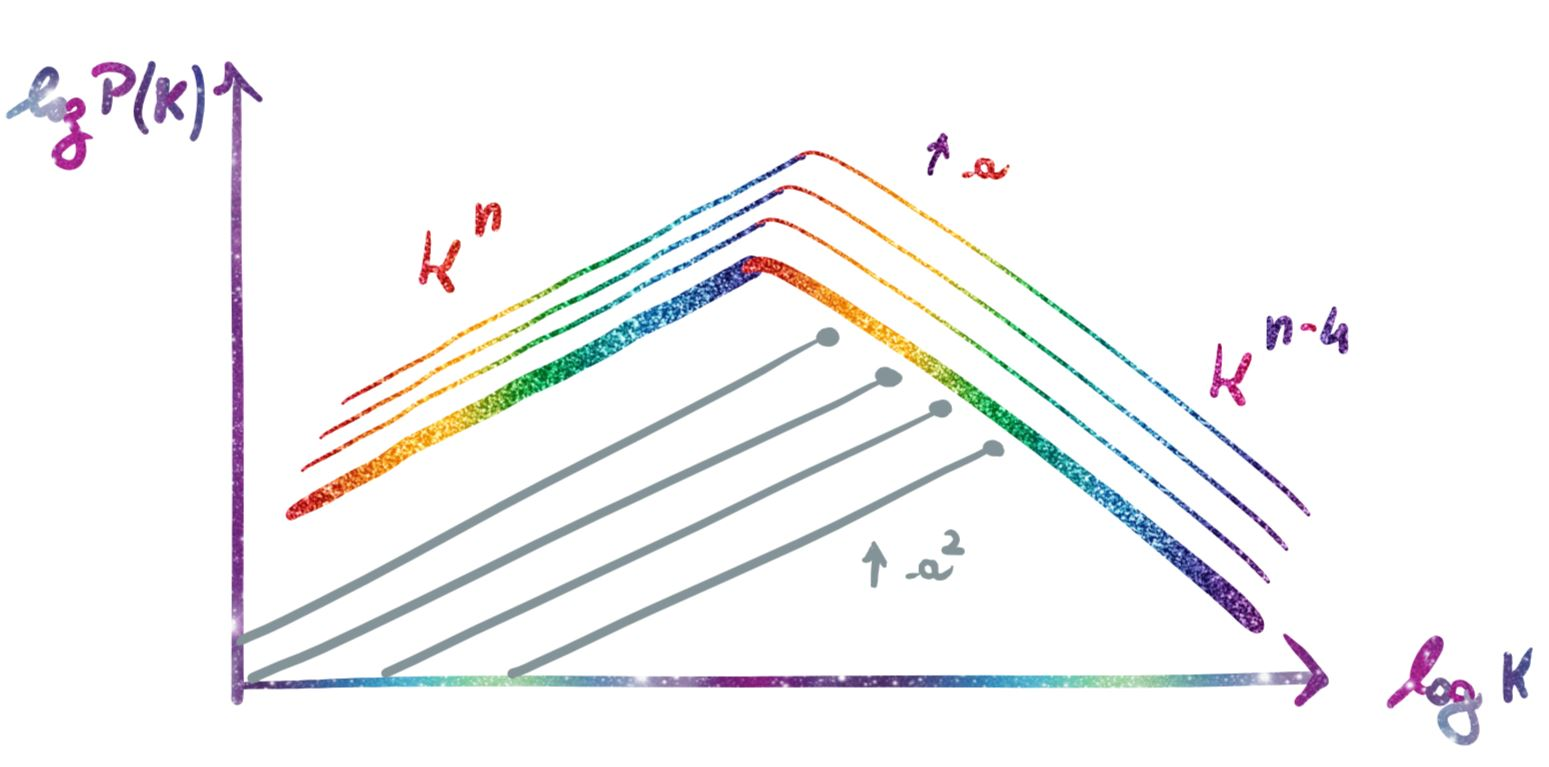
\includegraphics[width=.8 \textwidth]{Pictures/8/pertmatevolnic.jpg}
    \caption{Evoluzione dello spettro di potenza per la materia. In grigio le fasi prima dell'equivalenza: le scale piccole ($k$ grandi) entrano via via nell'orizzonte e stagnano. L'orizzonte si muove verso sinistra $\leftarrowtail $. In arcobaleno glitterato lo spettro al momento dell'equivalenza e successivamente la sua evoluzione autosimilare (come mai il picco si sposta un po' a destra?).} \label{fig8:bella} 
\end{figure}


La scala su cui avviene il turnover corrisponde a quella che entra nell'orizzonte al momento dell'equivalenza $k_{eq}$, pertanto lo spettro di potenza è influenzato anche dal valore di $\Omega_{m0}$. Studiando gli andamenti si ha: $k_{eq}\propto R_H^{-1}(t_{eq}) \propto \dot{a} = a H_0 E = f(H_0,\Omega_{m0})$. Inoltre come visto in precedenza: $1+z_{eq}=\Omega_{m0}/\Omega_{R0}$. Pertanto con più materia l'equivalenza avviene a redshift più alti con la conseguenza che l'orizzonte riesce a inglobare meno $k$: si preserva maggiormente lo spettro primordiale e il turnover si sposta a destra $\rightarrowtail $ (Fig. \ref{fig8:bella2}). Per un ragionamento analogo, all'aumentare della componente radiativa (e.g. neutrini) il picco si sposta a sinistra $\leftarrowtail $. Osservativamente, $k_{eq}\simeq 2\cdot 10^{-2}\; h$ Mpc$^{-1}$.
\begin{figure}[H]
    \centering
    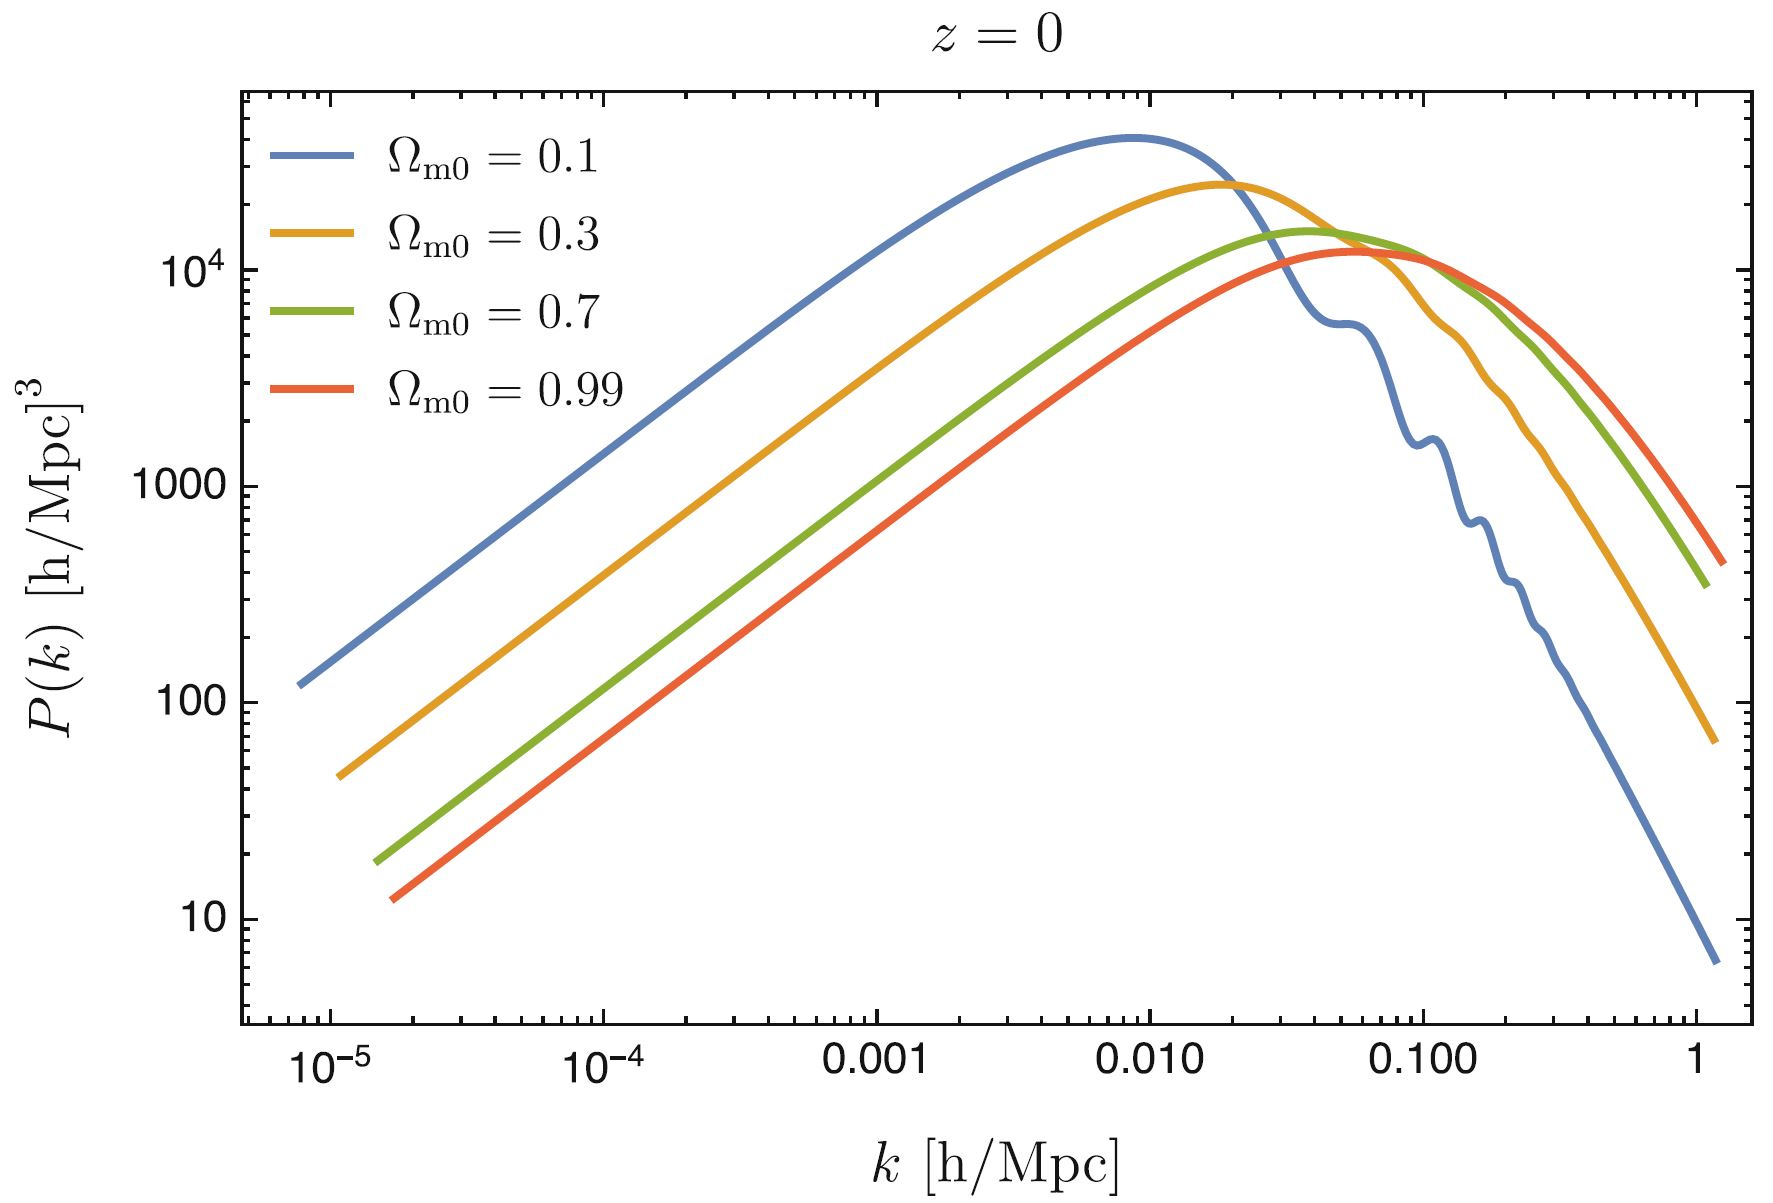
\includegraphics[width=.6 \textwidth]{Pictures/8/pertmatevol.jpg}
    \caption{Spettro di potenza per la materia al variare di $\Omega_{m0}$. Da: Oliver Piattella - \textit{Lecture notes in Cosmology} (Springer, 2018)}\label{fig8:bella2} 
\end{figure}

Per misurare $n$ bisogna osservare la curva per $k<k_{eq}$, che non è modificata dalla microfisica. Gli ammassi di galassie si collocano a destra del picco in corrispondenza $n_{eff}\approx 0$ e in seguito si trovano le galassie con $n_{eff}\approx -1$. Lo spettro osservato tramite survey di galassie e ammassi (Fig. \ref{fig8:bella3}) rigetta il modello HDM (così come fa la CMB). Modelli con $n\neq 1$ sono detti \textit{tilted}, e.g. per $n=0.8$ (meno ripidi) si sposta potenza sulle grandi scale, sfavorendo il collasso di piccole strutture.

\begin{figure}[H]
    \subfloat[]{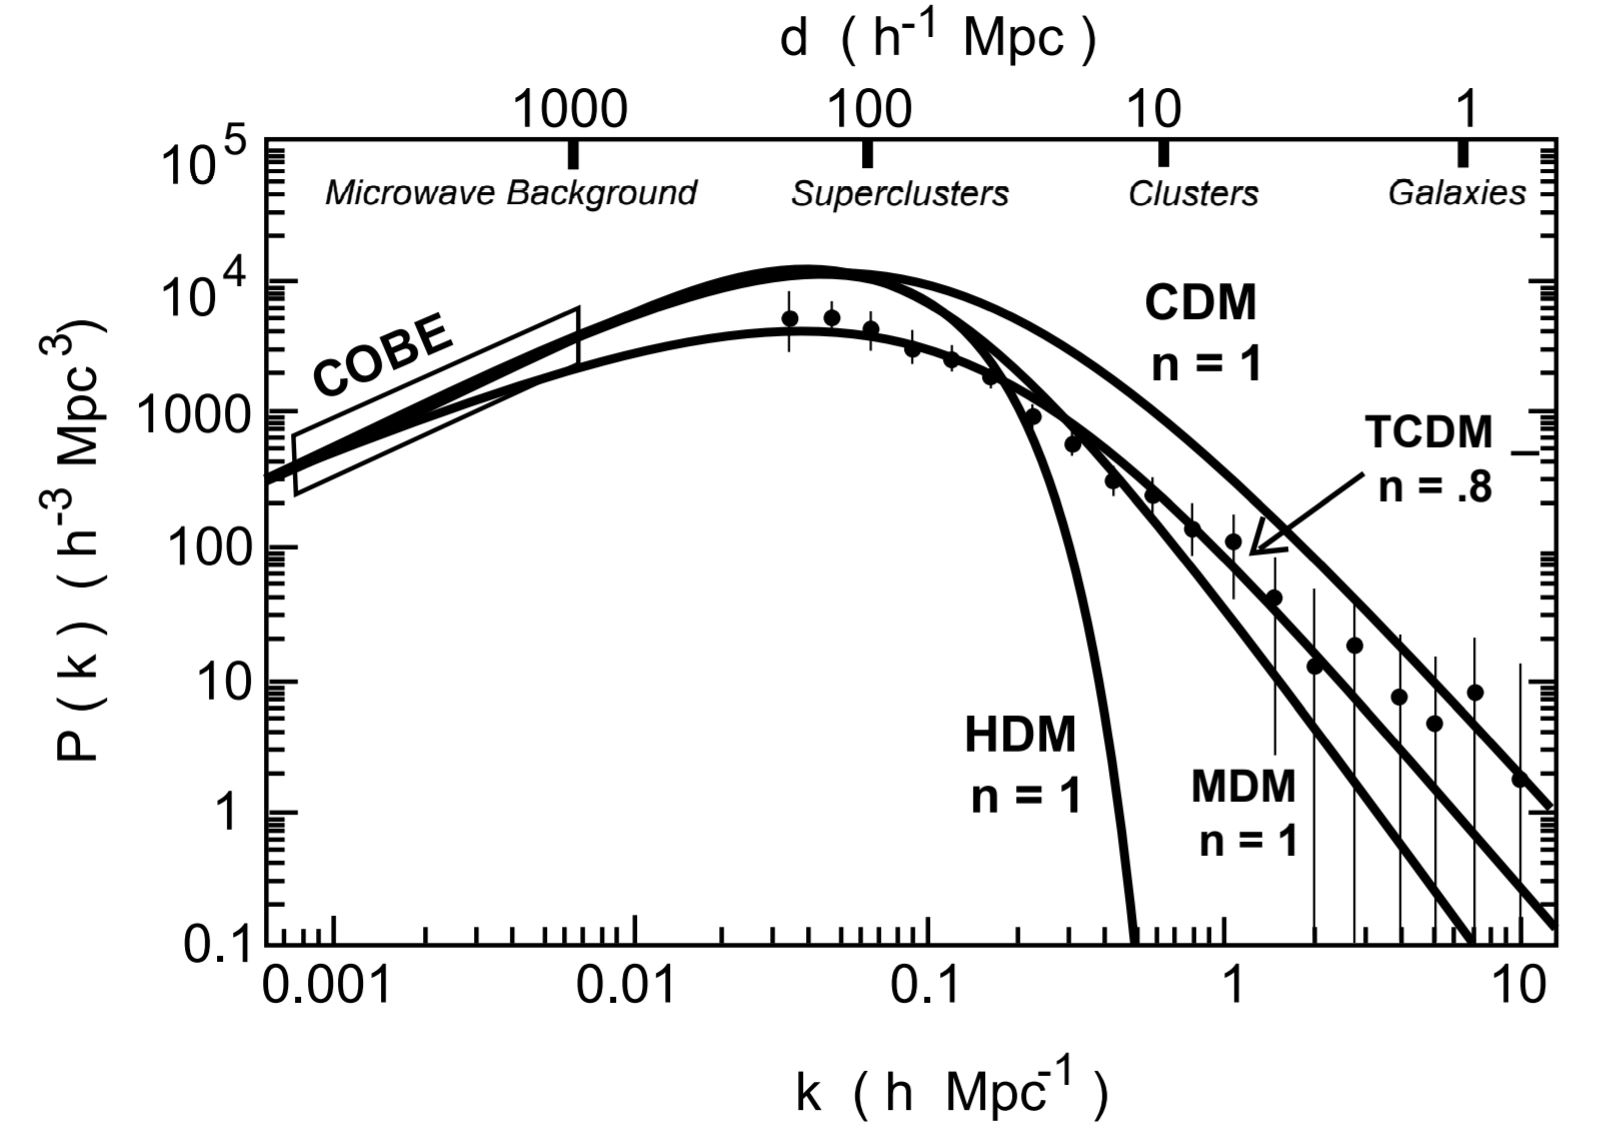
\includegraphics[width=.6\textwidth]{Pictures/8/tris1.jpg}}$\;\;$
    \subfloat[]{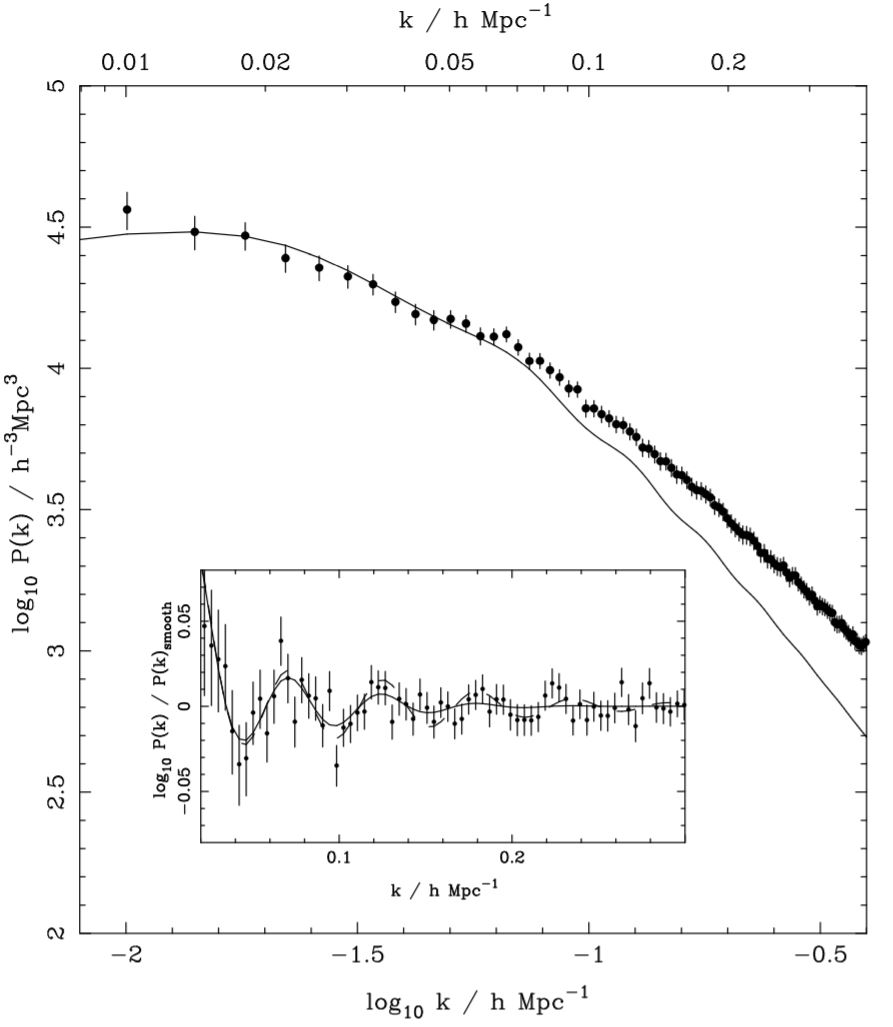
\includegraphics[width=.355\textwidth]{Pictures/8/tris3.jpg}}
    \caption{(a) Modelli di densità di potenza per Hot, Mixed (Warm) e Cold Dark Matter (i punti rappresentano i dati osservati che fittano un modello \textit{tilted}) (From: Kolb - \textit{Particle Physics in the Early Universe}, 1998); (b) Redshift-space power spectrum (notare $k/h$ sulle ascisse) per un campione di galassie (From: Percival et al. - \textit{The shape of the SDSS DR5 galaxy power spectrum}, 2006).} \label{fig8:bella3} 
\end{figure}


\subsection{Effetto del \textit{free-streaming}}
Mediante un'analisi più dettagliata si nota che per il modello HDM la densità di potenza decade per $k$ grandi e il turnover è spostato leggermente a destra rispetto al CDM (questo secondo effetto si notava in un'immagine a bassa qualità che è stata rigettata dall'editore). Questo è dovuto al fatto che $M_{fs, HDM}\simeq 10^{16}M_\odot$ (vs. $M_{fs, CDM}< 10^{6}M_\odot$), pertanto le perturbazioni sono state cancellate per scale maggiori o $k$ più piccoli (il taglio dovuto al free streaming per il modello CDM è fuori dal grafico a destra, non è rilevante cosmologicamente). Inoltre, lo shift a destra del picco è dovuto al fatto che il free streaming è causale e può avvenire solo dentro l'orizzonte. 

Un modo alternativo per visualizzare questo effetto è fare uso della quantità adimensionale $k^3\mathcal{P}(k)$. Ancor meglio, a voler essere precisi, in letteratura si fa uso della quantità:
\begin{equation}
    \Delta^2(k) = \frac{k^3}{2\pi^2}\mathcal{P}(k)
\end{equation}
che è la vera \textbf{potenza} delle perturbazioni (si usa anche la sua radice). Deviazioni dal modello CDM per grandi $k$, possono essere imputate alla presenza di neutrini massicci, pertanto se ne può stimare la loro massa media (misurando da qui $\rho_\nu$ e dalla CMB $N_\nu$). Lo stesso ragionamento vale nel caso di warm dark matter (Fig. \ref{fig8:bella4}).


\begin{figure}[H]
    \centering
    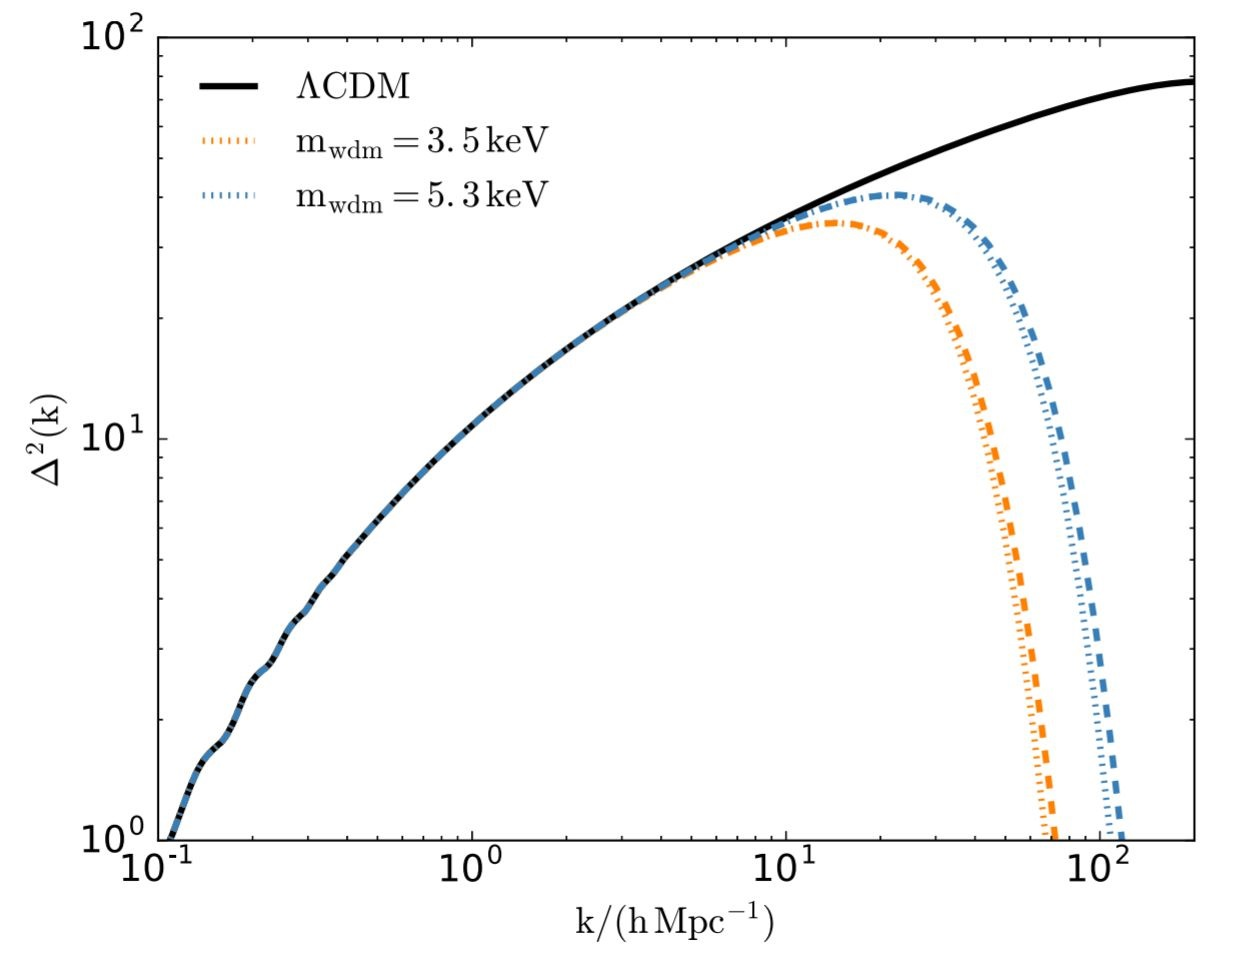
\includegraphics[width=.53 \textwidth]{Pictures/8/tris4.jpg}
    \vspace*{-1em}
    \caption{Spettro di potenza per modelli $\Lambda$CDM e WDM. $\Lambda$CDM: $k^3\mathcal{P}(k)\propto 1$ per $k$ grandi, R e M piccoli; $k^3\mathcal{P}(k)\propto k^4$ per $k$ piccoli, R e M grandi.  (From: Ricaldi et al. - \textit{On general features of warm dark matter with reduced relativistic
    gas}, 2018).} \label{fig8:bella4}
\end{figure}

\begin{example}[Funzione di trasferimento] 
    In letteratura si fa spesso uso della seguente convenzione:
    \begin{equation}
        \mathcal{P}(t_{eq},k)=\mathcal{P}_i(k)\; T^2(k)
    \end{equation}
    dove $T(k)$ è la funzione di trasferimento e nel caso in analisi è costante prima dell'equivalenza ed evolve $\propto k^{-2}$ dopo. Questa quantità dipende molto dalle assunzioni sulla materia oscura (Fig. \ref{fig8:transfun}) e sulla cosmologia, mentre $\mathcal{P}_i$ dipende dal modello inflazionario. Inoltre per il regime non lineare la trattazione viene ulteriormente complicata.

\end{example}
\begin{figure}[H]
    \centering
    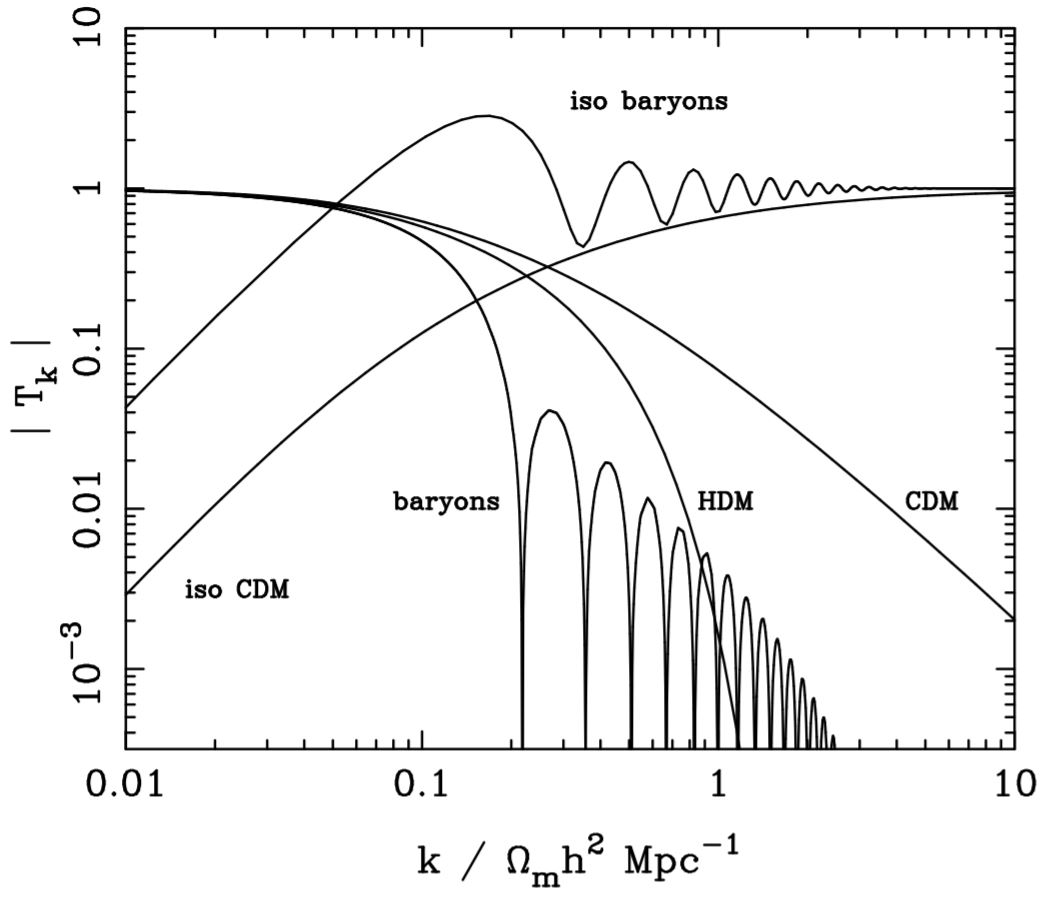
\includegraphics[width=.53 \textwidth]{Pictures/8/transfun.jpg}
    \vspace*{-1em}
    \caption{Funzione di trasferimento per vari modelli Si noti che $T_k\to 1$ a piccoli $k$ per modelli adiabatici e a grandi $k$ per modelli a isocurvatura. Per la dark matter il numero d'onda caratteristico scala proporzionalmente a $\Omega_m h^2$, i barioni hanno un comportamento diverso come verrà discusso a breve. Infine si può notare che la HDM è in difetto di potenza rispetto alla CDM. (From: J.A. Peacock - \textit{Large-scale surveys and cosmic structure}, 2003))}\label{fig8:transfun} 
\end{figure}



\subsection{Evoluzione post-equivalenza}
La figura \ref{fig8:bella} mostra l'evoluzione dello spettro di potenza anche dopo $t_{eq}$ per le assunzioni fino ad ora adottate. La crescita è \textit{autosimilare}. Questo non è più vero quando le perturbazioni diventano non lineari, ossia quando viene raggiunto il valore $\delta, \sigma_M \to 1$. Le scale piccole ($k$ grandi) diventano non lineari prima delle altre (cfr. Eq. \ref{eq8:sigmamvsr}). L’effetto netto è quello di un innalzamento dello spettro a grandi $k$ (Fig. \ref{fig8:ultimabella}).

\begin{figure}[H]
    \centering
    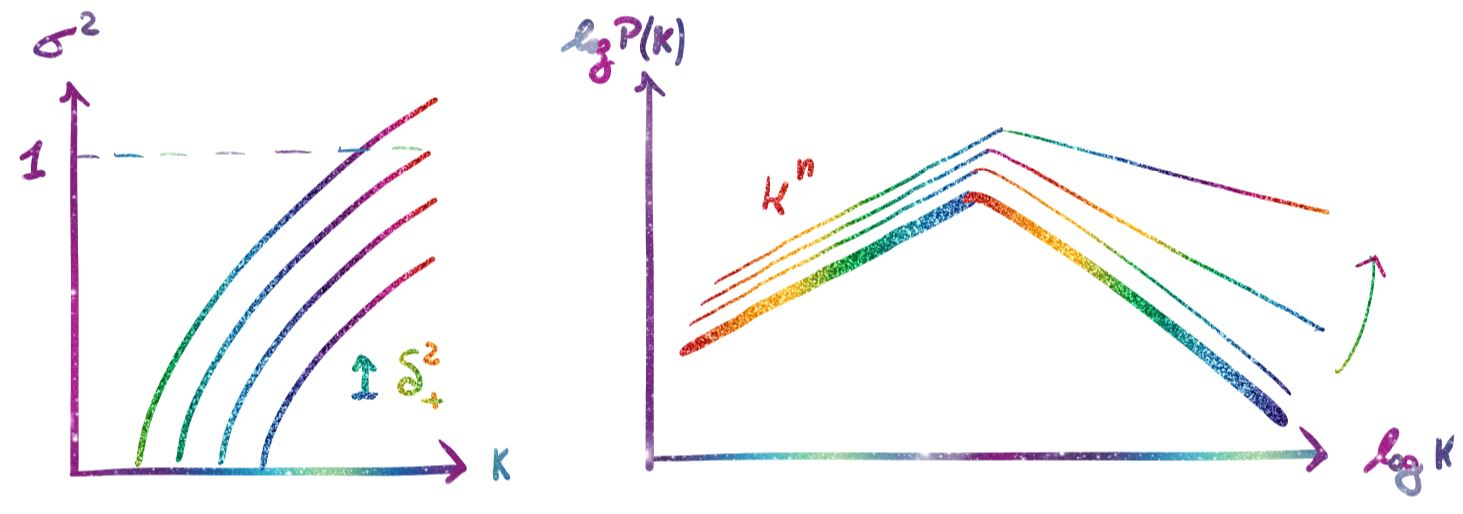
\includegraphics[width=.85 \textwidth]{Pictures/8/truevol.jpg}
    \vspace*{-1em}
    \caption{Sinistra: evoluzione di $\sigma^2$ in teoria lineare, le prime scale a diventare non lineari sono quelle grandi ($k$ piccoli); Destra: Crescita delle perturbazioni in regime non lineare. Lo spettro viene deformato a piccole scale, questo è un altro motivo per cui è meglio studiarlo a  grandi scale.}\label{fig8:ultimabella}
\end{figure}


\section{Distribuzione delle perturbazioni}
Come visto inizialmente si assume una distribuzione delle perturbazioni gaussiana:
\begin{equation}
    P(\delta_M)=\frac{1}{\sqrt{2\pi \sigma_M^2}}e^{-\frac{\delta_M^2}{2\sigma_M^2}}
\end{equation}
purtuttavia esiste un limite fisico per $\delta$ (ossia $\rho \geq 0$):
\begin{equation}
    \delta = \frac{\rho - \overbar{\rho}}{\overbar{\rho}} = \frac{\rho}{\overbar{\rho}}-1 > -1
\end{equation}
La situazione diventa ancora più imbarazzante col tempo perché la gaussiana si allargherebbe ($\sigma_M^2 \to \sigma_M^2 \delta_+^2$) ben oltre il valore limite $-1$. Per ovviare a questo problema si assume che la probabilità si accumuli vicino a $-1$ senza superarlo, rendendo di fatto la distribuzione non gaussiana. Col tempo la gaussiana si abbassa e si allarga, ma lo fa in modo asimmetrico (Fig. \ref{fig8:ultima}). Questa assunzione prevede una grande quantità di regioni sottodense (vuoti), mentre la materia si accumula tutta nei nodi. Questo discorso è valido su scale molto grandi, cioè quelle che hanno mantenuto la distribuzione gaussiana generata all’inflazione e per redshift elevati in cui la crescita è stata lineare su tutte le scale (CMB).

\vspace{1em}
L'\textbf{altezza delle perturbazioni} 
\begin{figure}[h]
    \centering
    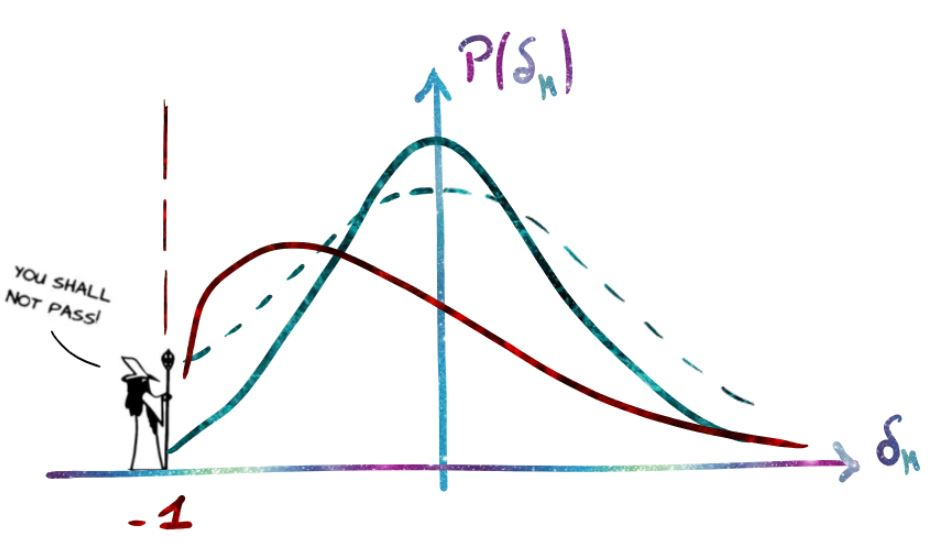
\includegraphics[width=.65 \textwidth]{Pictures/8/pdfevol.jpg}
    \vspace*{-1em}
    \caption{In verde tratteggiato l'evoluzione classica delle perturbazioni gaussiane. In rosso l'evoluzione assunta per evitare valori inferiori a $-1$. L'area sottesa non deve cambiare (=1), pertanto la distribuzione viene distorta.}\label{fig8:ultima}
\end{figure}

